\section{}
% A film crew is shooting a movie and performs a tracking shot, which involves a moving camera
% that follows a subject. In this case the camera is situated on a wheeled cart, and the crew
% encounters a small bump on the road which causes the camera to oscillate vertically.
% The total distance to be travelled by the camera is 40 m, with the length of each section shown
% below, and the combined mass of the camera and the cart is 210 kg. Assume the cart moves at a
% constant speed 𝑣 for the entire duration, and the height of the bump 𝑌 is 5 cm.
% 0
% a) (5 pts) Fortunately, the footage recorded while the camera moves on the bump will not be
% used in the final production, but the crew does not want any oscillations to occur after the
% camera cart has cleared the bump. If the entire tracking shot is to be filmed over 10
% seconds, determine the required wheel suspension stiffness 𝑘.
% b) (5 pts) The production crew tries refilming the shot with a camera speed of 𝑣/2. In
% reference to the indicated coordinate 𝑥, determine the displacement (𝑥) and velocity 𝑥
% ˙
% ( )
% of the camera at the end of the shot (ie. at 40 m). Assume that the stiffness 𝑘 corresponds
% to the answer in part a).

\textit{A film crew is shooting a movie and performs a tracking shot, which involves a moving camera that follows a subject. In this case the camera is situated on a wheeled cart, and the crew encounters a small bump on the road which causes the camera to oscillate vertically. The total distance to be travelled by the camera is 40 m, with the length of each section shown below, and the combined mass of the camera and the cart is 210 kg. Assume the cart moves at a constant speed $v$ for the entire duration, and the height of the bump $Y$ is 5 cm.}

\begin{figure}[H]
    \centering
    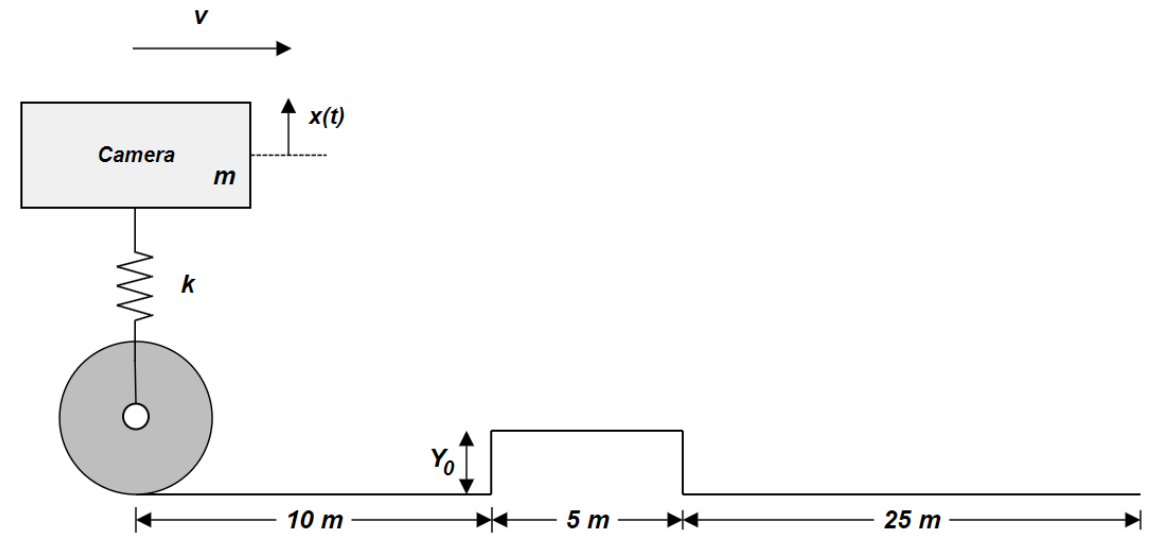
\includegraphics[width=0.8\linewidth]{Questions/Figures/Q2 Problem Diagram.png}
\end{figure}

\begin{enumerate}[label=(\alph*)]
    \item \textit{Fortunately the footage recorded while the camera moves on the bump will not be used in the final production, but the crew does not want any oscillations to occur after the camera cart has cleared the bump. If the entire tracking shot is to be filmed over 10 seconds, determine the required wheel suspension stiffness $k$.}
    \item \textit{The production crew tries refilming the shot with a camera speed of $v/2$. In reference to the indicated coordinate $x$, determine the displacement $(x)$ and velocity $\dot{x}$ of the camera at the end of the shot (i.e. at 40 m). Assume that the stiffness $k$ corresponds to the answer in part (a).}
\end{enumerate}

\subsection*{Solution}
\subsection{}
Assume that the cart's vertical displacement follows the ground exactly. Then at 10m, the forces on the camera are:
\begin{figure}[H]
    \centering
    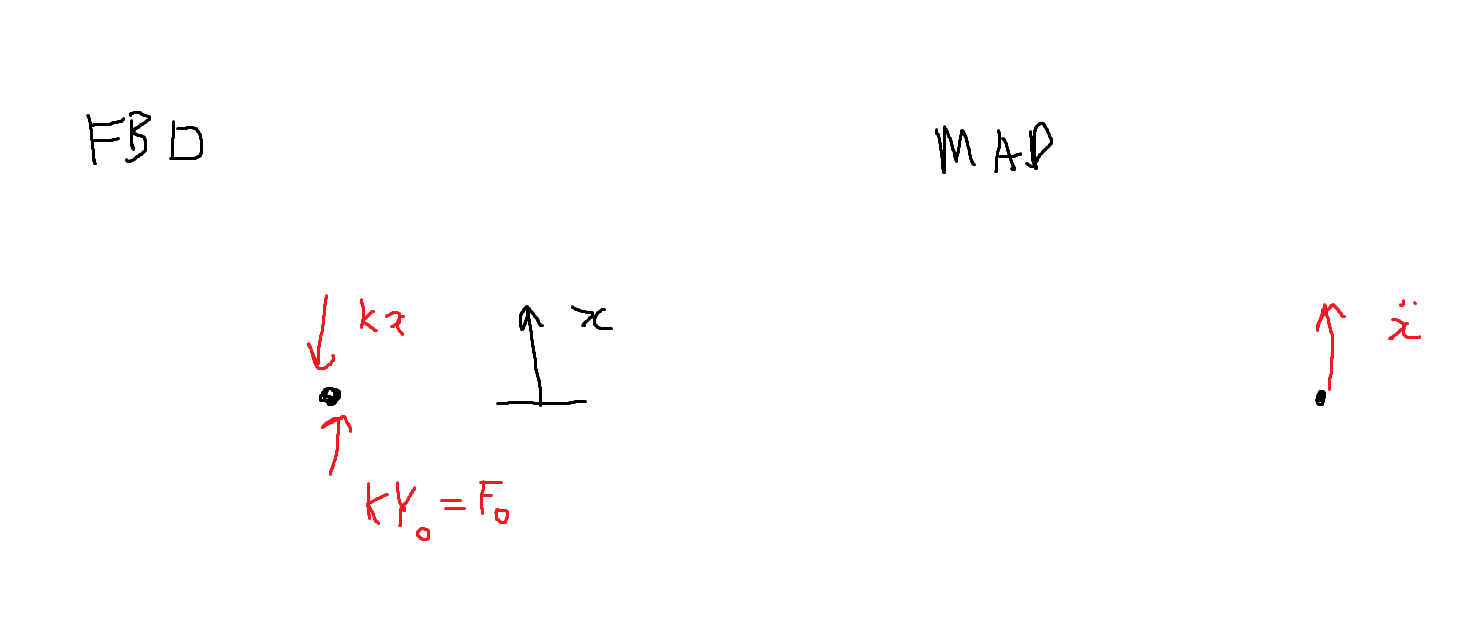
\includegraphics[width=0.8\linewidth]{Questions/Figures/Q2 FBD and MAD.png}
    \caption{Free body diagram and mass acceleration diagram.}
\end{figure}
Define $t$ as the time when the cart is at 10m. The initial conditions the time when the cart is at 10m, are:
\begin{align*}
    x(0) = 0, \quad \dot{x}(0) = 0 
\end{align*}
From Eq. (7.3), the solution is given by:
\begin{align*}
    x(t) &= \frac{F_0}{k} \left(1 - \cos(p t)\right) \\
    &= Y_0 \left(1 - \cos(p t)\right)
\end{align*}
From the textbook, we want to unload the cart at $t_2 = \frac{2 \pi}{p}$ since this will be the time when the camera has zero displacement and zero velocity. We can solve for $k$ using the following equation:
\begin{align*}
    t_2 &= \frac{2 \pi}{p} \\
    t_{2}^2 &= \frac{4 \pi^2}{k/m} \\
    \implies k &= \frac{4 \pi^2 m}{t_{2}^2}
\end{align*}
The time it takes for the cart to travel to the end of the bump is
\begin{align*}
    t_2 &= \frac{5}{v} 
\end{align*}
Then $k$ is 
\begin{align*}
    k &= \frac{4 \pi^2 m}{\left(\frac{5}{v}\right)^2} \\
    &= \boxed{\frac{4 \pi^2 m v^2}{25}}
\end{align*}

\subsection{}
In part a), we found stiffness such that 
\begin{align*}
    \tau &= \frac{2\pi}{p} = t_{2} = \frac{5}{v}
\end{align*}
Halving the speed of the cart will double the time it takes to travel the bump. The new time is then,
\begin{align*}
    t_{2b} &= \frac{5}{v/2} = \frac{10}{v} = \frac{4\pi}{p} = 2\tau
\end{align*}
This means it will take 2 periods of oscillation for the cart to travel the bump. But at every integer multiple of $\tau$, the displacement and velocity of the cart will be zero. Therefore, the displacement and velocity of the cart at the end of the bump will be zero.

After the bump, the system remains at zero displacement and velocity since there are no more forces acting on the cart. Therefore, the displacement and velocity of the cart at the end of the shot will be zero.
\begin{figure}[h]
    \centering
    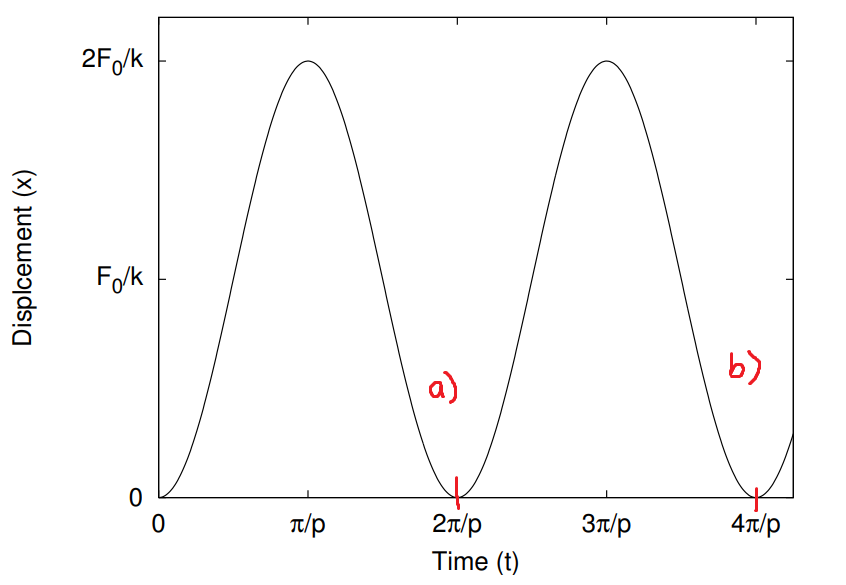
\includegraphics[width=0.5\linewidth]{Questions/Figures/Q2 Plot.png}
    \caption{Displacement plot. Halving speed of the cart places it at $t = 4\pi/p$.}
\end{figure}
\begin{empheq}[box=\fbox]{align*}
    x(t_{40m}) &= 0 \\
    \dot{x}(t_{40m}) &= 0
\end{empheq}